\documentclass{article}
\usepackage{iclr2026_conference,times}
%%%%% NEW MATH DEFINITIONS %%%%%

\usepackage{amsmath,amsfonts,bm}

% Mark sections of captions for referring to divisions of figures
\newcommand{\figleft}{{\em (Left)}}
\newcommand{\figcenter}{{\em (Center)}}
\newcommand{\figright}{{\em (Right)}}
\newcommand{\figtop}{{\em (Top)}}
\newcommand{\figbottom}{{\em (Bottom)}}
\newcommand{\captiona}{{\em (a)}}
\newcommand{\captionb}{{\em (b)}}
\newcommand{\captionc}{{\em (c)}}
\newcommand{\captiond}{{\em (d)}}

% Highlight a newly defined term
\newcommand{\newterm}[1]{{\bf #1}}


% Figure reference, lower-case.
\def\figref#1{figure~\ref{#1}}
% Figure reference, capital. For start of sentence
\def\Figref#1{Figure~\ref{#1}}
\def\twofigref#1#2{figures \ref{#1} and \ref{#2}}
\def\quadfigref#1#2#3#4{figures \ref{#1}, \ref{#2}, \ref{#3} and \ref{#4}}
% Section reference, lower-case.
\def\secref#1{section~\ref{#1}}
% Section reference, capital.
\def\Secref#1{Section~\ref{#1}}
% Reference to two sections.
\def\twosecrefs#1#2{sections \ref{#1} and \ref{#2}}
% Reference to three sections.
\def\secrefs#1#2#3{sections \ref{#1}, \ref{#2} and \ref{#3}}
% Reference to an equation, lower-case.
\def\eqref#1{equation~\ref{#1}}
% Reference to an equation, upper case
\def\Eqref#1{Equation~\ref{#1}}
% A raw reference to an equation---avoid using if possible
\def\plaineqref#1{\ref{#1}}
% Reference to a chapter, lower-case.
\def\chapref#1{chapter~\ref{#1}}
% Reference to an equation, upper case.
\def\Chapref#1{Chapter~\ref{#1}}
% Reference to a range of chapters
\def\rangechapref#1#2{chapters\ref{#1}--\ref{#2}}
% Reference to an algorithm, lower-case.
\def\algref#1{algorithm~\ref{#1}}
% Reference to an algorithm, upper case.
\def\Algref#1{Algorithm~\ref{#1}}
\def\twoalgref#1#2{algorithms \ref{#1} and \ref{#2}}
\def\Twoalgref#1#2{Algorithms \ref{#1} and \ref{#2}}
% Reference to a part, lower case
\def\partref#1{part~\ref{#1}}
% Reference to a part, upper case
\def\Partref#1{Part~\ref{#1}}
\def\twopartref#1#2{parts \ref{#1} and \ref{#2}}

\def\ceil#1{\lceil #1 \rceil}
\def\floor#1{\lfloor #1 \rfloor}
\def\1{\bm{1}}
\newcommand{\train}{\mathcal{D}}
\newcommand{\valid}{\mathcal{D_{\mathrm{valid}}}}
\newcommand{\test}{\mathcal{D_{\mathrm{test}}}}

\def\eps{{\epsilon}}


% Random variables
\def\reta{{\textnormal{$\eta$}}}
\def\ra{{\textnormal{a}}}
\def\rb{{\textnormal{b}}}
\def\rc{{\textnormal{c}}}
\def\rd{{\textnormal{d}}}
\def\re{{\textnormal{e}}}
\def\rf{{\textnormal{f}}}
\def\rg{{\textnormal{g}}}
\def\rh{{\textnormal{h}}}
\def\ri{{\textnormal{i}}}
\def\rj{{\textnormal{j}}}
\def\rk{{\textnormal{k}}}
\def\rl{{\textnormal{l}}}
% rm is already a command, just don't name any random variables m
\def\rn{{\textnormal{n}}}
\def\ro{{\textnormal{o}}}
\def\rp{{\textnormal{p}}}
\def\rq{{\textnormal{q}}}
\def\rr{{\textnormal{r}}}
\def\rs{{\textnormal{s}}}
\def\rt{{\textnormal{t}}}
\def\ru{{\textnormal{u}}}
\def\rv{{\textnormal{v}}}
\def\rw{{\textnormal{w}}}
\def\rx{{\textnormal{x}}}
\def\ry{{\textnormal{y}}}
\def\rz{{\textnormal{z}}}

% Random vectors
\def\rvepsilon{{\mathbf{\epsilon}}}
\def\rvtheta{{\mathbf{\theta}}}
\def\rva{{\mathbf{a}}}
\def\rvb{{\mathbf{b}}}
\def\rvc{{\mathbf{c}}}
\def\rvd{{\mathbf{d}}}
\def\rve{{\mathbf{e}}}
\def\rvf{{\mathbf{f}}}
\def\rvg{{\mathbf{g}}}
\def\rvh{{\mathbf{h}}}
\def\rvu{{\mathbf{i}}}
\def\rvj{{\mathbf{j}}}
\def\rvk{{\mathbf{k}}}
\def\rvl{{\mathbf{l}}}
\def\rvm{{\mathbf{m}}}
\def\rvn{{\mathbf{n}}}
\def\rvo{{\mathbf{o}}}
\def\rvp{{\mathbf{p}}}
\def\rvq{{\mathbf{q}}}
\def\rvr{{\mathbf{r}}}
\def\rvs{{\mathbf{s}}}
\def\rvt{{\mathbf{t}}}
\def\rvu{{\mathbf{u}}}
\def\rvv{{\mathbf{v}}}
\def\rvw{{\mathbf{w}}}
\def\rvx{{\mathbf{x}}}
\def\rvy{{\mathbf{y}}}
\def\rvz{{\mathbf{z}}}

% Elements of random vectors
\def\erva{{\textnormal{a}}}
\def\ervb{{\textnormal{b}}}
\def\ervc{{\textnormal{c}}}
\def\ervd{{\textnormal{d}}}
\def\erve{{\textnormal{e}}}
\def\ervf{{\textnormal{f}}}
\def\ervg{{\textnormal{g}}}
\def\ervh{{\textnormal{h}}}
\def\ervi{{\textnormal{i}}}
\def\ervj{{\textnormal{j}}}
\def\ervk{{\textnormal{k}}}
\def\ervl{{\textnormal{l}}}
\def\ervm{{\textnormal{m}}}
\def\ervn{{\textnormal{n}}}
\def\ervo{{\textnormal{o}}}
\def\ervp{{\textnormal{p}}}
\def\ervq{{\textnormal{q}}}
\def\ervr{{\textnormal{r}}}
\def\ervs{{\textnormal{s}}}
\def\ervt{{\textnormal{t}}}
\def\ervu{{\textnormal{u}}}
\def\ervv{{\textnormal{v}}}
\def\ervw{{\textnormal{w}}}
\def\ervx{{\textnormal{x}}}
\def\ervy{{\textnormal{y}}}
\def\ervz{{\textnormal{z}}}

% Random matrices
\def\rmA{{\mathbf{A}}}
\def\rmB{{\mathbf{B}}}
\def\rmC{{\mathbf{C}}}
\def\rmD{{\mathbf{D}}}
\def\rmE{{\mathbf{E}}}
\def\rmF{{\mathbf{F}}}
\def\rmG{{\mathbf{G}}}
\def\rmH{{\mathbf{H}}}
\def\rmI{{\mathbf{I}}}
\def\rmJ{{\mathbf{J}}}
\def\rmK{{\mathbf{K}}}
\def\rmL{{\mathbf{L}}}
\def\rmM{{\mathbf{M}}}
\def\rmN{{\mathbf{N}}}
\def\rmO{{\mathbf{O}}}
\def\rmP{{\mathbf{P}}}
\def\rmQ{{\mathbf{Q}}}
\def\rmR{{\mathbf{R}}}
\def\rmS{{\mathbf{S}}}
\def\rmT{{\mathbf{T}}}
\def\rmU{{\mathbf{U}}}
\def\rmV{{\mathbf{V}}}
\def\rmW{{\mathbf{W}}}
\def\rmX{{\mathbf{X}}}
\def\rmY{{\mathbf{Y}}}
\def\rmZ{{\mathbf{Z}}}

% Elements of random matrices
\def\ermA{{\textnormal{A}}}
\def\ermB{{\textnormal{B}}}
\def\ermC{{\textnormal{C}}}
\def\ermD{{\textnormal{D}}}
\def\ermE{{\textnormal{E}}}
\def\ermF{{\textnormal{F}}}
\def\ermG{{\textnormal{G}}}
\def\ermH{{\textnormal{H}}}
\def\ermI{{\textnormal{I}}}
\def\ermJ{{\textnormal{J}}}
\def\ermK{{\textnormal{K}}}
\def\ermL{{\textnormal{L}}}
\def\ermM{{\textnormal{M}}}
\def\ermN{{\textnormal{N}}}
\def\ermO{{\textnormal{O}}}
\def\ermP{{\textnormal{P}}}
\def\ermQ{{\textnormal{Q}}}
\def\ermR{{\textnormal{R}}}
\def\ermS{{\textnormal{S}}}
\def\ermT{{\textnormal{T}}}
\def\ermU{{\textnormal{U}}}
\def\ermV{{\textnormal{V}}}
\def\ermW{{\textnormal{W}}}
\def\ermX{{\textnormal{X}}}
\def\ermY{{\textnormal{Y}}}
\def\ermZ{{\textnormal{Z}}}

% Vectors
\def\vzero{{\bm{0}}}
\def\vone{{\bm{1}}}
\def\vmu{{\bm{\mu}}}
\def\vtheta{{\bm{\theta}}}
\def\va{{\bm{a}}}
\def\vb{{\bm{b}}}
\def\vc{{\bm{c}}}
\def\vd{{\bm{d}}}
\def\ve{{\bm{e}}}
\def\vf{{\bm{f}}}
\def\vg{{\bm{g}}}
\def\vh{{\bm{h}}}
\def\vi{{\bm{i}}}
\def\vj{{\bm{j}}}
\def\vk{{\bm{k}}}
\def\vl{{\bm{l}}}
\def\vm{{\bm{m}}}
\def\vn{{\bm{n}}}
\def\vo{{\bm{o}}}
\def\vp{{\bm{p}}}
\def\vq{{\bm{q}}}
\def\vr{{\bm{r}}}
\def\vs{{\bm{s}}}
\def\vt{{\bm{t}}}
\def\vu{{\bm{u}}}
\def\vv{{\bm{v}}}
\def\vw{{\bm{w}}}
\def\vx{{\bm{x}}}
\def\vy{{\bm{y}}}
\def\vz{{\bm{z}}}

% Elements of vectors
\def\evalpha{{\alpha}}
\def\evbeta{{\beta}}
\def\evepsilon{{\epsilon}}
\def\evlambda{{\lambda}}
\def\evomega{{\omega}}
\def\evmu{{\mu}}
\def\evpsi{{\psi}}
\def\evsigma{{\sigma}}
\def\evtheta{{\theta}}
\def\eva{{a}}
\def\evb{{b}}
\def\evc{{c}}
\def\evd{{d}}
\def\eve{{e}}
\def\evf{{f}}
\def\evg{{g}}
\def\evh{{h}}
\def\evi{{i}}
\def\evj{{j}}
\def\evk{{k}}
\def\evl{{l}}
\def\evm{{m}}
\def\evn{{n}}
\def\evo{{o}}
\def\evp{{p}}
\def\evq{{q}}
\def\evr{{r}}
\def\evs{{s}}
\def\evt{{t}}
\def\evu{{u}}
\def\evv{{v}}
\def\evw{{w}}
\def\evx{{x}}
\def\evy{{y}}
\def\evz{{z}}

% Matrix
\def\mA{{\bm{A}}}
\def\mB{{\bm{B}}}
\def\mC{{\bm{C}}}
\def\mD{{\bm{D}}}
\def\mE{{\bm{E}}}
\def\mF{{\bm{F}}}
\def\mG{{\bm{G}}}
\def\mH{{\bm{H}}}
\def\mI{{\bm{I}}}
\def\mJ{{\bm{J}}}
\def\mK{{\bm{K}}}
\def\mL{{\bm{L}}}
\def\mM{{\bm{M}}}
\def\mN{{\bm{N}}}
\def\mO{{\bm{O}}}
\def\mP{{\bm{P}}}
\def\mQ{{\bm{Q}}}
\def\mR{{\bm{R}}}
\def\mS{{\bm{S}}}
\def\mT{{\bm{T}}}
\def\mU{{\bm{U}}}
\def\mV{{\bm{V}}}
\def\mW{{\bm{W}}}
\def\mX{{\bm{X}}}
\def\mY{{\bm{Y}}}
\def\mZ{{\bm{Z}}}
\def\mBeta{{\bm{\beta}}}
\def\mPhi{{\bm{\Phi}}}
\def\mLambda{{\bm{\Lambda}}}
\def\mSigma{{\bm{\Sigma}}}

% Tensor
\DeclareMathAlphabet{\mathsfit}{\encodingdefault}{\sfdefault}{m}{sl}
\SetMathAlphabet{\mathsfit}{bold}{\encodingdefault}{\sfdefault}{bx}{n}
\newcommand{\tens}[1]{\bm{\mathsfit{#1}}}
\def\tA{{\tens{A}}}
\def\tB{{\tens{B}}}
\def\tC{{\tens{C}}}
\def\tD{{\tens{D}}}
\def\tE{{\tens{E}}}
\def\tF{{\tens{F}}}
\def\tG{{\tens{G}}}
\def\tH{{\tens{H}}}
\def\tI{{\tens{I}}}
\def\tJ{{\tens{J}}}
\def\tK{{\tens{K}}}
\def\tL{{\tens{L}}}
\def\tM{{\tens{M}}}
\def\tN{{\tens{N}}}
\def\tO{{\tens{O}}}
\def\tP{{\tens{P}}}
\def\tQ{{\tens{Q}}}
\def\tR{{\tens{R}}}
\def\tS{{\tens{S}}}
\def\tT{{\tens{T}}}
\def\tU{{\tens{U}}}
\def\tV{{\tens{V}}}
\def\tW{{\tens{W}}}
\def\tX{{\tens{X}}}
\def\tY{{\tens{Y}}}
\def\tZ{{\tens{Z}}}


% Graph
\def\gA{{\mathcal{A}}}
\def\gB{{\mathcal{B}}}
\def\gC{{\mathcal{C}}}
\def\gD{{\mathcal{D}}}
\def\gE{{\mathcal{E}}}
\def\gF{{\mathcal{F}}}
\def\gG{{\mathcal{G}}}
\def\gH{{\mathcal{H}}}
\def\gI{{\mathcal{I}}}
\def\gJ{{\mathcal{J}}}
\def\gK{{\mathcal{K}}}
\def\gL{{\mathcal{L}}}
\def\gM{{\mathcal{M}}}
\def\gN{{\mathcal{N}}}
\def\gO{{\mathcal{O}}}
\def\gP{{\mathcal{P}}}
\def\gQ{{\mathcal{Q}}}
\def\gR{{\mathcal{R}}}
\def\gS{{\mathcal{S}}}
\def\gT{{\mathcal{T}}}
\def\gU{{\mathcal{U}}}
\def\gV{{\mathcal{V}}}
\def\gW{{\mathcal{W}}}
\def\gX{{\mathcal{X}}}
\def\gY{{\mathcal{Y}}}
\def\gZ{{\mathcal{Z}}}

% Sets
\def\sA{{\mathbb{A}}}
\def\sB{{\mathbb{B}}}
\def\sC{{\mathbb{C}}}
\def\sD{{\mathbb{D}}}
% Don't use a set called E, because this would be the same as our symbol
% for expectation.
\def\sF{{\mathbb{F}}}
\def\sG{{\mathbb{G}}}
\def\sH{{\mathbb{H}}}
\def\sI{{\mathbb{I}}}
\def\sJ{{\mathbb{J}}}
\def\sK{{\mathbb{K}}}
\def\sL{{\mathbb{L}}}
\def\sM{{\mathbb{M}}}
\def\sN{{\mathbb{N}}}
\def\sO{{\mathbb{O}}}
\def\sP{{\mathbb{P}}}
\def\sQ{{\mathbb{Q}}}
\def\sR{{\mathbb{R}}}
\def\sS{{\mathbb{S}}}
\def\sT{{\mathbb{T}}}
\def\sU{{\mathbb{U}}}
\def\sV{{\mathbb{V}}}
\def\sW{{\mathbb{W}}}
\def\sX{{\mathbb{X}}}
\def\sY{{\mathbb{Y}}}
\def\sZ{{\mathbb{Z}}}

% Entries of a matrix
\def\emLambda{{\Lambda}}
\def\emA{{A}}
\def\emB{{B}}
\def\emC{{C}}
\def\emD{{D}}
\def\emE{{E}}
\def\emF{{F}}
\def\emG{{G}}
\def\emH{{H}}
\def\emI{{I}}
\def\emJ{{J}}
\def\emK{{K}}
\def\emL{{L}}
\def\emM{{M}}
\def\emN{{N}}
\def\emO{{O}}
\def\emP{{P}}
\def\emQ{{Q}}
\def\emR{{R}}
\def\emS{{S}}
\def\emT{{T}}
\def\emU{{U}}
\def\emV{{V}}
\def\emW{{W}}
\def\emX{{X}}
\def\emY{{Y}}
\def\emZ{{Z}}
\def\emSigma{{\Sigma}}

% entries of a tensor
% Same font as tensor, without \bm wrapper
\newcommand{\etens}[1]{\mathsfit{#1}}
\def\etLambda{{\etens{\Lambda}}}
\def\etA{{\etens{A}}}
\def\etB{{\etens{B}}}
\def\etC{{\etens{C}}}
\def\etD{{\etens{D}}}
\def\etE{{\etens{E}}}
\def\etF{{\etens{F}}}
\def\etG{{\etens{G}}}
\def\etH{{\etens{H}}}
\def\etI{{\etens{I}}}
\def\etJ{{\etens{J}}}
\def\etK{{\etens{K}}}
\def\etL{{\etens{L}}}
\def\etM{{\etens{M}}}
\def\etN{{\etens{N}}}
\def\etO{{\etens{O}}}
\def\etP{{\etens{P}}}
\def\etQ{{\etens{Q}}}
\def\etR{{\etens{R}}}
\def\etS{{\etens{S}}}
\def\etT{{\etens{T}}}
\def\etU{{\etens{U}}}
\def\etV{{\etens{V}}}
\def\etW{{\etens{W}}}
\def\etX{{\etens{X}}}
\def\etY{{\etens{Y}}}
\def\etZ{{\etens{Z}}}

% The true underlying data generating distribution
\newcommand{\pdata}{p_{\rm{data}}}
% The empirical distribution defined by the training set
\newcommand{\ptrain}{\hat{p}_{\rm{data}}}
\newcommand{\Ptrain}{\hat{P}_{\rm{data}}}
% The model distribution
\newcommand{\pmodel}{p_{\rm{model}}}
\newcommand{\Pmodel}{P_{\rm{model}}}
\newcommand{\ptildemodel}{\tilde{p}_{\rm{model}}}
% Stochastic autoencoder distributions
\newcommand{\pencode}{p_{\rm{encoder}}}
\newcommand{\pdecode}{p_{\rm{decoder}}}
\newcommand{\precons}{p_{\rm{reconstruct}}}

\newcommand{\laplace}{\mathrm{Laplace}} % Laplace distribution

\newcommand{\E}{\mathbb{E}}
\newcommand{\Ls}{\mathcal{L}}
\newcommand{\R}{\mathbb{R}}
\newcommand{\emp}{\tilde{p}}
\newcommand{\lr}{\alpha}
\newcommand{\reg}{\lambda}
\newcommand{\rect}{\mathrm{rectifier}}
\newcommand{\softmax}{\mathrm{softmax}}
\newcommand{\sigmoid}{\sigma}
\newcommand{\softplus}{\zeta}
\newcommand{\KL}{D_{\mathrm{KL}}}
\newcommand{\Var}{\mathrm{Var}}
\newcommand{\standarderror}{\mathrm{SE}}
\newcommand{\Cov}{\mathrm{Cov}}
% Wolfram Mathworld says $L^2$ is for function spaces and $\ell^2$ is for vectors
% But then they seem to use $L^2$ for vectors throughout the site, and so does
% wikipedia.
\newcommand{\normlzero}{L^0}
\newcommand{\normlone}{L^1}
\newcommand{\normltwo}{L^2}
\newcommand{\normlp}{L^p}
\newcommand{\normmax}{L^\infty}

\newcommand{\parents}{Pa} % See usage in notation.tex. Chosen to match Daphne's book.

\DeclareMathOperator*{\argmax}{arg\,max}
\DeclareMathOperator*{\argmin}{arg\,min}

\DeclareMathOperator{\sign}{sign}
\DeclareMathOperator{\Tr}{Tr}
\let\ab\allowbreak

\usepackage{amsmath}
\usepackage{booktabs}
\usepackage{graphicx}
\usepackage{microtype}
\usepackage{hyperref}
\usepackage{url}

\title{When Does Symmetric Source Pairing Help Flow Policies for Robot Control?}

\author{Anonymous authors}

% \iclrfinalcopy
\begin{document}
\maketitle

\begin{abstract}
Flow-matching robot policies generate actions by integrating a learned vector
field from a source sample, making test-time source selection part of the
deployed controller. We study a simple, training-free rule that averages the
two action endpoints produced from a Gaussian source and its exact negation.
At equal total neural-function evaluations, this symmetric projection recovers
$0.945\pm0.059$ return (mean$\pm$SD across four independently trained Unitree
Go2 policies) relative to the official random-source rule; the policy-level
95\% Student-$t$ interval is $[0.852,1.038]$, while the conservative exact
one-sided sign-test value is $0.0625$. Across the same policies, symmetric
pairing also exceeds two-source IID averaging by $0.566$ return at equal pair
compute. Mechanism measurements show near-opposite source-conditioned action
displacements (mean cosine $-0.969$) and a residual RMS ratio of $0.124$, versus
$0.710$ for IID averaging. A batched implementation is 1.19$\times$ faster
than sequential pairing and, at batch 4096 on an H200, is faster than one
64-step random solve. Strong controls delimit the result: deterministic
zero-source inference matches or exceeds symmetric pairing, the
symmetry-specific advantage does not resolve on Spot, and mirrored closed-loop
rollouts fail a preregistered variance-reduction gate. Symmetric pairing is
therefore a reliable correction for stochastic-source degradation on these Go2
policies, not a universally superior deployment rule.
\end{abstract}

\section{Introduction}

Flow and diffusion policies represent complex action distributions through an
iterative generative process rather than a simple parametric likelihood
\citep{chi2023diffusionpolicy,lipman2022flowmatching}. Flow Policy Optimization
(FPO) and FPO++ extend this representation to online policy-gradient training
without exact action likelihoods \citep{mcallister2025flowpolicy,yi2026flowcontrol}.
Their flexibility introduces a deployment choice that does not arise for a
deterministic policy: from which source should the action flow be integrated?
The official FPO++ evaluation uses either a fresh Gaussian source or a zero
source, and reports that the latter often performs better. This gap matters
scientifically because it reveals that part of the learned stochastic action
variation degrades return, and practically because source selection changes
both behavior and solver cost without retraining.

We ask a narrow question: can a symmetric source construction remove the
harmful component of stochastic inference while preserving a controlled amount
of flow-policy averaging? Given the endpoint map $F_\theta(o,z)$ for observation
$o$ and source $z$, we evaluate
\begin{equation}
  a_{\mathrm{sym}}(o,z)
  = \tfrac{1}{2}\left[F_\theta(o,z)+F_\theta(o,-z)\right].
  \label{eq:symmetric}
\end{equation}
This is the classical antithetic construction applied to conditional policy
endpoints. Antithetic sources and approximate affine antisymmetry are already
established for generative models \citep{jia2025antithetic}; our goal is not to
reintroduce them. Instead, we determine what survives in closed-loop robot
control under equal-compute, deterministic, IID-averaging, cross-policy, and
cross-task controls.

The central result is deliberately qualified. Across four independently
trained Go2 policies, symmetric projection consistently recovers the official
random-source return deficit at equal total solver evaluations. Direct endpoint
measurements connect this recovery to cancellation of a dominant source-odd
action displacement. However, zero-source inference is at least as strong, and
on Spot the data do not separate symmetric pairing from generic two-endpoint
averaging. A further attempt to use mirrored sources as a closed-loop return
control variate fails. The evidence supports a robust diagnostic and correction
for one stochastic-inference failure mode, not a new state of the art.

Our contribution is a controlled account of this phenomenon: (i) policy-level
replication across four Go2 training seeds with equal-total-NFE and equal-pair-NFE
comparisons; (ii) a source-parity mechanism audit and a batched throughput
implementation; and (iii) deterministic, Spot, and mirrored-rollout controls
that expose where the appealing local symmetry does not translate into a
stronger deployment policy. All analyses read archived evaluation records, and
the appendix maps every reported number to a committed artifact.

\section{Background and inference rules}

\subsection{Flow policies}

Flow matching learns a time-dependent vector field that transports a simple
source distribution to a target data distribution
\citep{lipman2022flowmatching,liu2022rectified}. In a conditional robot policy,
the vector field is conditioned on observation $o$. Starting at
$x_0=z\sim\mathcal{N}(0,I)$, an ODE solver produces the endpoint
$F_\theta(o,z)=x_1$, which is interpreted as the action. FPO replaces explicit
action-likelihood ratios with ratios derived from conditional flow-matching
losses, while FPO++ adds per-sample ratios and an asymmetric trust region to
stabilize robot-control training \citep{mcallister2025flowpolicy,yi2026flowcontrol}.
These training details remain unchanged in our study: every comparison uses a
frozen official FPO++ policy.

\subsection{Controlled source selection}

Table~\ref{tab:rules} defines the four inference rules. Random and zero use one
endpoint. IID-pair and symmetric inference average two endpoints, differing
only in whether the second source is independent or the exact negative of the
first. We count one vector-field evaluation per Euler step and explicitly
match total NFE when making compute claims. In particular, two 32-step
symmetric endpoints and one 64-step random endpoint both cost 64 NFE per
action. The equal-pair attribution comparison uses 64 steps for both endpoints
in both IID and symmetric methods, for 128 total NFE.

\begin{table}[t]
  \caption{Frozen-policy inference rules. $z,w\stackrel{\mathrm{iid}}{\sim}
  \mathcal{N}(0,I)$ and $F^{K}$ denotes an Euler solve with $K$ steps.}
  \label{tab:rules}
  \centering
  \small
  \begin{tabular}{lclc}
    \toprule
    Rule & Action & Endpoints & Total NFE \\
    \midrule
    zero64 & $F^{64}(o,0)$ & 1 & 64 \\
    random64 & $F^{64}(o,z)$ & 1 & 64 \\
    IID-pair32 & $[F^{32}(o,z)+F^{32}(o,w)]/2$ & 2 & 64 \\
    symmetric32 & $[F^{32}(o,z)+F^{32}(o,-z)]/2$ & 2 & 64 \\
    IID-pair64 & $[F^{64}(o,z)+F^{64}(o,w)]/2$ & 2 & 128 \\
    symmetric64 & $[F^{64}(o,z)+F^{64}(o,-z)]/2$ & 2 & 128 \\
    \bottomrule
  \end{tabular}
\end{table}

\subsection{Source-parity diagnostic}

Let $D(o,z)=F_\theta(o,z)-F_\theta(o,0)$ be the source-conditioned displacement
from the zero-source endpoint. Its even and odd components are
\begin{equation}
 D_{\mathrm{even}}(o,z)=\tfrac{1}{2}[D(o,z)+D(o,-z)],\quad
 D_{\mathrm{odd}}(o,z)=\tfrac{1}{2}[D(o,z)-D(o,-z)].
\end{equation}
Symmetric projection leaves only $D_{\mathrm{even}}$. We report the cosine
between $D(o,z)$ and $D(o,-z)$ and the normalized residual
$\lVert D_{\mathrm{even}}\rVert_{\mathrm{RMS}}/
\lVert D(o,z)\rVert_{\mathrm{RMS}}$. A small residual indicates an
approximately affine, source-antisymmetric endpoint map. The corresponding IID
ratio replaces $-z$ with an independent $w$ and tests whether cancellation is
specific to symmetry rather than averaging alone.

\section{Experimental design}

\subsection{Tasks, policies, and paired evaluation}

We use the official IsaacLab FPO++ locomotion setup
\citep{yi2026flowcontrol}. Go2 experiments train four policies with seeds
42--45, each for 1500 iterations with 4096 parallel environments and the
released hyperparameters. We evaluate the fixed final checkpoint
\texttt{model\_1499.pt}; no run is excluded and no checkpoint is selected by
evaluation return. The primary independent unit for cross-policy claims is the
training seed, not the thousands of nested simulator episodes.

Within a policy, comparisons are paired by initial environment state. Random,
IID-pair, and symmetric modes share the complete primary source stream; IID
uses a separately seeded secondary stream. The three new Go2 policies use 512
episodes per method for the 128-NFE attribution evaluation and 256 episodes per
method for the equal-total-NFE evaluation. Seed 42 uses the corresponding
locked 256-episode studies. All validity gates require equal initial-observation
hashes, expected endpoint counts and NFE, finite returns, and unchanged actor
parameters.

For cross-task evaluation, we train one official Spot seed-42 policy for 1500
iterations and evaluate its fixed final checkpoint in five paired cells:
zero64, zero32, random64, IID-pair32, and symmetric32. Each cell contains 256
episodes, for 1280 valid episodes total. This experiment was designed as an
attribution test: transfer requires both a positive symmetric-minus-random
interval and a positive symmetric-minus-IID interval.

\subsection{Statistics}

For generalization across Go2 policies, we compute the paired return difference
within each training seed and summarize the four seed effects using their mean,
sample SD, and a two-sided 95\% Student-$t$ interval with three degrees of
freedom. Because four seeds are too few to assess normality, we additionally
report the exact one-sided sign-test value. Four same-direction effects yield
$p=1/16=0.0625$; we do not describe this as conventionally significant.
Within-policy comparisons use the preregistered paired bootstrap with 20,000
resamples. Spot intervals likewise resample paired episode indices. The
mirrored-rollout variance ratio uses 20,000 paired bootstrap resamples. All
interval definitions and statistical units are stated with their results.

\section{Results}

\begin{figure*}[t]
  \centering
  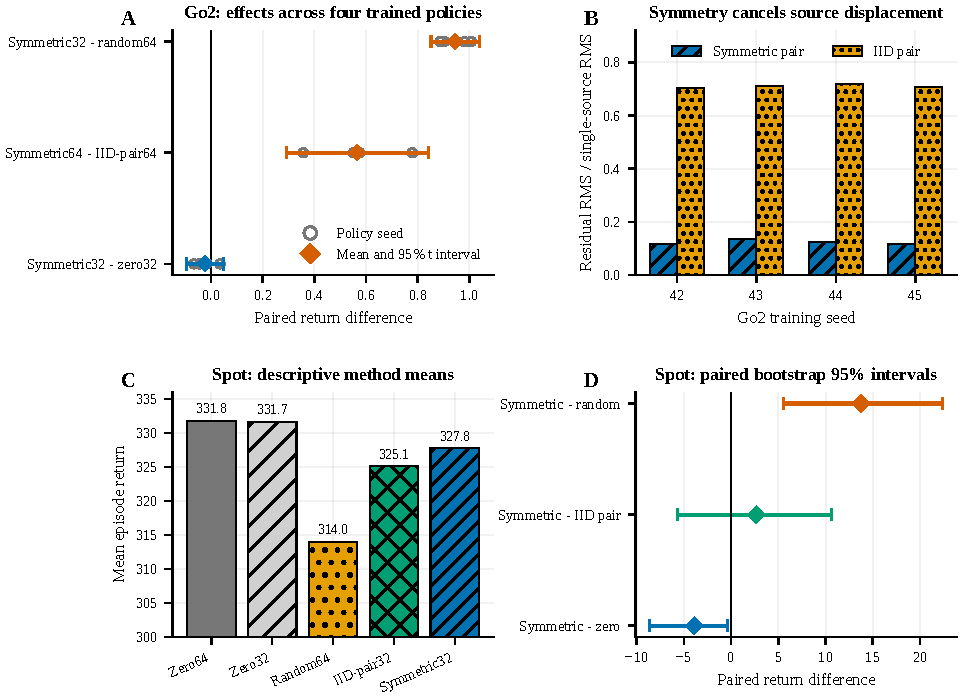
\includegraphics[width=\textwidth]{figures/fig_main_results.pdf}
  \caption{Core results and controls. \textbf{A}: paired Go2 return effects
  across four independently trained policies. Open circles are training-seed
  effects; diamonds and bars are the policy-level mean and two-sided 95\%
  Student-$t$ interval ($n=4$ policies). The first and third comparisons use
  equal 64 total NFE; the second uses equal 128 total NFE.
  \textbf{B}: normalized endpoint residuals for exact symmetric and IID pairs
  on 128 environments over eight rollout steps per policy; lower is stronger
  cancellation. \textbf{C}: descriptive Spot means from five paired cells of
  256 episodes. \textbf{D}: Spot paired return differences with 20,000-sample
  bootstrap 95\% intervals. Symmetry recovers the random-source deficit on
  both tasks, but does not beat zero source and is not separated from IID
  averaging on Spot.}
  \label{fig:main}
\end{figure*}

\subsection{Symmetric projection recovers the Go2 random-source deficit}

Figure~\ref{fig:main}A shows the equal-total-NFE comparison. Symmetric32 minus
random64 is positive for all four policies: $0.981$, $0.903$, $1.008$, and
$0.888$. The mean effect is $0.945$ return with SD $0.059$ and policy-level
95\% $t$ interval $[0.852,1.038]$. The magnitude is stable across independently
trained policies, although the exact sign-test value remains $0.0625$ because
$n=4$.

The stronger attribution comparison holds pair compute fixed. Symmetric64
minus IID-pair64 is also positive for all four policies, with effects $0.779$,
$0.357$, $0.574$, and $0.551$. Its mean is $0.566$ (SD $0.173$), with
policy-level interval $[0.291,0.840]$ and exact one-sided sign-test
$p=0.0625$. Generic two-endpoint averaging therefore does not fully explain
the Go2 recovery.

Deterministic deployment changes the conclusion. Symmetric32 minus zero32 has
mean $-0.023$ (SD $0.044$) and interval $[-0.094,0.047]$. Thus symmetric
projection repairs the official stochastic inference rule, but it does not
improve on the stronger deterministic zero-source control.

\subsection{The endpoint map is approximately affine antisymmetric}

Across the same four policies, the cosine between $D(o,z)$ and $D(o,-z)$ is
$-0.969$ on average (range $-0.972$ to $-0.964$). The symmetric residual ratio
is $0.124$ (range $0.118$--$0.136$), whereas the IID residual ratio is $0.710$
(range $0.702$--$0.718$); Figure~\ref{fig:main}B shows that this gap is present
for every policy. In absolute units, the even-component RMS is $0.0386$ and the
odd-component RMS is $0.3088$. The source effect is therefore dominated by an
odd component that exact pairing removes. This evidence closely matches the
affine-antisymmetry account reported for other generative models
\citep{jia2025antithetic}, now measured in conditional robot actions rather
than images or uncertainty estimators.

\subsection{Spot shows recovery without symmetry-specific attribution}

On Spot, random64 obtains mean return $314.00$, IID-pair32 $325.11$,
symmetric32 $327.78$, zero32 $331.70$, and zero64 $331.81$
(Figure~\ref{fig:main}C). Symmetric32 exceeds random64 by $13.78$ with paired
bootstrap interval $[5.58,22.37]$. The improvement relative to IID-pair32 is
only $2.67$, with interval $[-5.72,10.66]$, so the locked symmetry-specific
transfer gate fails. Symmetric32 is also worse than zero32 by $-3.92$, interval
$[-8.60,-0.42]$. The cross-task result supports a broader two-endpoint
averaging benefit relative to random inference, but cannot attribute that
benefit specifically to exact source negation.

\subsection{Batched inference removes the policy-only latency penalty}

\begin{figure}[t]
  \centering
  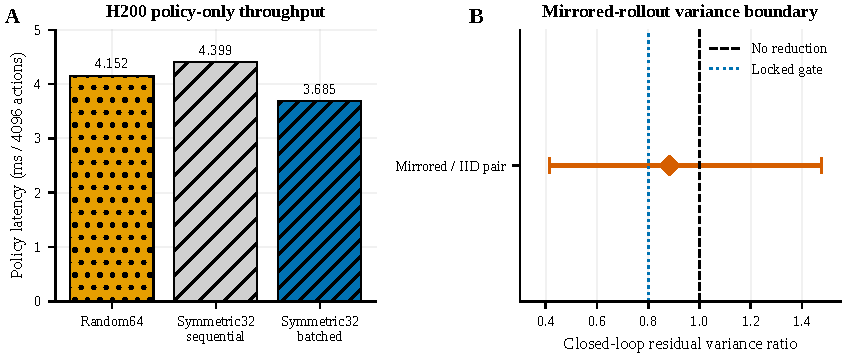
\includegraphics[width=\linewidth]{figures/fig_efficiency_boundary.pdf}
  \caption{Efficiency and failure boundary. \textbf{A}: median policy-only
  latency for 4096 frozen Go2 observations on one H200, after 10 warm-ups and
  over five blocks of 20 synchronized calls. This is neither end-to-end
  simulator latency nor single-robot latency. \textbf{B}: mirrored-to-IID
  closed-loop pair-residual variance ratio with a 20,000-sample bootstrap 95\%
  interval. The interval crosses the no-reduction line and the point estimate
  misses the locked 0.80 gate.}
  \label{fig:efficiency}
\end{figure}

Concatenating observations and the $z/-z$ sources along the batch dimension
computes both 32-step endpoints in one doubled policy call. On an H200 at batch
4096, random64 takes $4.152$ ms, sequential symmetric32 takes $4.399$ ms, and
batched symmetric32 takes $3.685$ ms (Figure~\ref{fig:efficiency}A). Batching is
$1.194\times$ faster than sequential pairing and uses $0.888\times$ the
random64 latency in this high-parallelism policy-only measurement. Batched and
sequential actions differ by at most $4.77\times10^{-7}$. The result shows that
equal NFE can translate into favorable accelerator throughput; it does not
establish latency on physical control hardware.

\subsection{Local symmetry does not survive as a reliable return control variate}

A natural extension is to execute $z$ and $-z$ in separate environments and
average their returns, as antithetic perturbations and common random numbers
can reduce variance in optimization or rollout comparison
\citep{salimans2017es,yu2018antithetic,yadav2026crn}. We preregistered a small
Go2 test using 256 paired environments and compared mirrored and IID return
residual variance. The mirrored/IID ratio is $0.882$, with bootstrap interval
$[0.414,1.475]$ (Figure~\ref{fig:efficiency}B), failing both the ratio-at-most
$0.80$ gate and the requirement that the upper bound be below one. The paired
returns remain positively correlated ($0.479$ for mirrored versus $0.450$ for
IID). Immediate action antisymmetry is therefore not preserved by closed-loop
dynamics strongly enough to support this training-control-variate extension.

\section{Related work}

\paragraph{Flow and diffusion policies.}
Flow matching trains continuous normalizing flows through vector-field
regression \citep{lipman2022flowmatching}; rectified flow emphasizes straight
transport paths and coarse integration \citep{liu2022rectified}. Generative
policies apply related iterative samplers to multimodal robot actions
\citep{chi2023diffusionpolicy}. FPO introduces a conditional-flow-matching
surrogate for policy optimization, and FPO++ makes it effective across
locomotion, motion tracking, and manipulation
\citep{mcallister2025flowpolicy,yi2026flowcontrol}. We leave training untouched
and isolate a test-time source-selection effect in frozen FPO++ policies.

\paragraph{Antithetic sampling and common randomness.}
Mirrored perturbations are widely used to reduce estimator variance, including
evolution strategies and bandit gradients
\citep{salimans2017es,yu2018antithetic}. Common random numbers similarly improve
comparisons between simulated rollouts under appropriate coupling assumptions
\citep{yadav2026crn}. Most directly, \citet{jia2025antithetic} show that $z/-z$
initial noises generate negatively correlated endpoints across diffusion and
other generative models, and propose approximate affine antisymmetry as the
mechanism. Our study adopts that established construction and asks a different
question: whether endpoint averaging improves closed-loop robot return under
equal-compute and deterministic controls. The Go2 result is positive, while
the Spot attribution and mirrored-rollout experiments mark important limits.

\section{Limitations}

The principal limitation is breadth. The policy-level result contains four
Go2 training seeds but only one Spot policy, and no H1, G1, manipulation, or
physical-robot confirmation. Four same-direction Go2 effects are encouraging,
yet the exact sign test cannot cross 0.05 with only four units. The Spot
interval against IID averaging is wide and crosses zero, so cross-task evidence
does not support a universal symmetry-specific effect.

The method is also not the best observed deployment rule. Zero-source inference
matches symmetric projection on Go2 and exceeds it on Spot. The practical value
is consequently diagnostic and conditional: symmetric projection preserves a
stochastic construction while cancelling a harmful source-odd component, but
applications that do not require stochastic source semantics should prefer the
validated zero-source baseline. Throughput was measured on one H200 at batch
4096; doubled batching may not help at low batch size or on embedded hardware.

Finally, the mechanism evidence is empirical. Approximate affine antisymmetry
explains immediate endpoint cancellation, but closed-loop feedback can alter
the observation distribution, as demonstrated by the failed mirrored-return
variance test. We do not claim a theorem connecting action-space parity to
long-horizon return.

\section{Conclusion}

Symmetric source pairing reliably recovers the stochastic-inference deficit of
flow-matching control policies across four independently trained Go2 agents at
equal compute. Endpoint audits identify a stable source-odd displacement that
exact pairing cancels, and accelerator batching makes the construction
efficient at official training parallelism. Just as importantly, deterministic
and cross-task controls prevent a broader conclusion: zero-source inference is
stronger, Spot does not isolate a symmetry-specific advantage, and mirrored
rollouts do not provide a reliable return control variate. These results turn
a visually compelling generative-model symmetry into a bounded, reproducible
robot-control finding rather than an overstated deployment method.

\section*{Broader impact}

This work concerns simulated locomotion policy evaluation and does not introduce
new physical-robot capability. More reliable source-selection diagnostics can
reduce wasted evaluation compute and discourage selecting a stochastic
inference rule without deterministic controls. Conversely, simulation returns
and high-batch GPU timing should not be interpreted as physical safety or
real-time deployment evidence. Any deployment should separately validate
latency, stability, and failure recovery on its target hardware.

\section*{LLM usage disclosure}

Language-model assistance was used to organize experiment records, draft text,
and generate plotting and build scripts. All numerical claims are produced from
committed experiment artifacts by deterministic scripts, and all cited metadata
was checked against arXiv or Crossref records. The authors remain responsible
for the claims, code, and final manuscript.

\bibliography{references}
\bibliographystyle{iclr2026_conference}

\appendix
\section{Reproducibility details}

\subsection{Artifact map}

Table~\ref{tab:artifacts} maps each result family to its frozen protocol,
analysis, and machine-readable record. All paths are relative to the repository
root. The figure script reads these JSON records directly and does not contain
hard-coded result values.

\begin{table}[h]
  \caption{Paper claims and committed artifact directories.}
  \label{tab:artifacts}
  \centering
  \small
  \begin{tabular}{ll}
    \toprule
    Claim & Artifact directory \\
    \midrule
    Four-policy return effects & \texttt{experiments/go2-antithetic-cross-policy-summary} \\
    Independent Go2 policies & \texttt{experiments/go2-antithetic-independent-seeds} \\
    Equal-total-NFE seed 42 & \texttt{experiments/go2-antithetic-equal-total-nfe} \\
    Affine antisymmetry & \texttt{experiments/go2-antithetic-affine-mechanism} \\
    H200 throughput & \texttt{experiments/go2-antithetic-batched-throughput} \\
    Spot control & \texttt{experiments/spot-antithetic-cross-task} \\
    Mirrored rollout boundary & \texttt{experiments/go2-mirrored-rollout-variance} \\
    \bottomrule
  \end{tabular}
\end{table}

\subsection{Implementation}

The inference helper accepts explicit source tensors. IID-pair inference returns
$[F(o,z)+F(o,w)]/2$; symmetric inference invokes the same helper with $(z,-z)$.
The batched version concatenates $(o,o)$ and $(z,-z)$, calls the unchanged policy
once, splits the resulting endpoints, and averages them in float32. Validation
checks source shape, floating-point type, finite values, endpoint shape, and the
expected doubled batch dimension. Unit tests verify exact negation, arithmetic
averaging, non-finite rejection, and single-call batching.

\subsection{Evaluation configuration}

All locomotion training uses 4096 environments and 1500 iterations. Evaluations
use one completed episode per environment. Go2 independent-policy attribution
uses 512 environments per method for seeds 43--45; equal-total-NFE evaluations
use 256. The source seed and initial-state pairing are fixed within each
experiment and recorded in its protocol and result JSON. Spot uses one seed-42
policy and five paired 256-environment cells. The mechanism audit uses 128
environments, eight rollout steps, and 32 solver steps for each of four
policies. The throughput audit uses ten warm-up calls followed by five rotated
blocks of 20 synchronized calls per method.

\subsection{Commands}

The paper figures and PDF can be rebuilt from the repository root with:
\begin{verbatim}
python3 paper/iclr2026/figures/gen_figures.py
latexmk -cd -pdf -interaction=nonstopmode \
  -halt-on-error paper/iclr2026/main.tex
\end{verbatim}
The experiment-specific remote entry scripts are under
\texttt{research\_scripts/remote/}; each protocol records the seeds, checkpoints,
environment counts, and pass/fail gates used before execution. A short
validation run should precede any remote rerun, as documented by the repository
workflow.

\section{Additional numerical results}

For the three new Go2 policies (seeds 43--45), the pooled stratified paired
bootstrap gain of symmetric64 over IID-pair64 is $0.494$, interval
$[0.353,0.642]$; the gain over random64 is $0.920$, interval
$[0.771,1.075]$. These intervals summarize paired episodes within the three
policies and are not substitutes for the policy-level uncertainty in the main
text. Symmetric64 minus zero64 is $-0.085$, interval $[-0.212,0.041]$.

For the source-parity audit, the average single-source displacement RMS is
$0.312$, the average opposite-source displacement RMS is $0.311$, the even RMS
is $0.0386$, and the odd RMS is $0.3088$. Every policy passes the locked cosine,
residual-ratio, exact-source-negation, finite-endpoint, and unchanged-parameter
checks.

The Spot zero32-minus-zero64 difference is $-0.110$, with paired bootstrap
interval $[-3.730,2.813]$. Thus reducing integration depth alone does not explain
the gap between stochastic random inference and the deterministic controls.

\end{document}
